\section {High-Level-Planner Node} \label{hl_node}

The \hlplanner\ node does the high-level control of the system, which also includes receiving search commands from the user. In Figure \ref{hl_execution} an overview of the execution of a search is given. After an description of the data structures used in the implementation the individual steps are described in more detail.

\begin{figure}
  \centering
  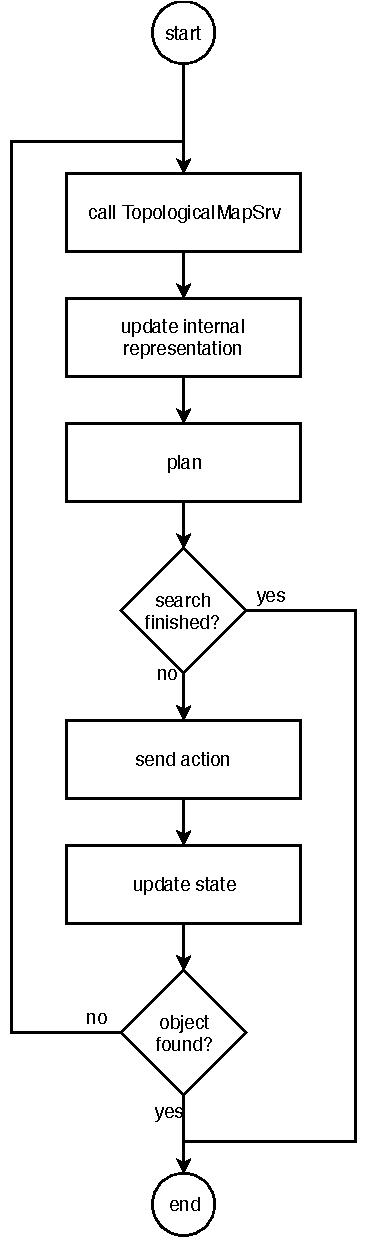
\includegraphics[width=0.4\textwidth,clip]{figures/hl_planner_execution.pdf}
  \caption[High-level planner execution overview]{High-level planner execution overview}
  \label{hl_execution}
\end{figure}

\subsection{Data Structures} \label{llimpl_data}

The \texttt{TopologicalMap} class stores the information of the topological map in a form which is easier to use by the planner. For every room the object probabilities, the times to completely search the room, and the expected search times are stored. Furthermore, for every pair of rooms the time to travel from room A to room B, the rooms on the way from A to B, and the poses of the doorways on the way are stored.  

\begin{minipage}{\linewidth}
\begin{lstlisting}[caption=TopologicalMap,frame=single, label=TopologicalMap]
   float[] object_probabilities
   float[] search_times
   float[] expected_search_times
   float[][] travel_times
   int[][][] travel_paths
   Pose[][][] travel_waypoints
\end{lstlisting}
\end{minipage}

The \texttt{Action} class specifies the high-level tasks. Its variables contain the information needed for the execution of the task. The \texttt{type} variable specifies what high-level task to execute, the \texttt{target{\_}object} and \texttt{target{\_}room} variables contain the searched object and the current room. In case of the move-through-doorway task the next room is stored in the \texttt{target{\_}room} variable and the \texttt{pose} variable contains the doorway pose.

\begin{minipage}{\linewidth}
\begin{lstlisting}[caption=Action,frame=single, label=Action]
   Type type
   int target_object
   int target_room
   Pose pose
\end{lstlisting}
\end{minipage}

The \texttt{State} class represents the current state of the search, storing the current room and which rooms are already visited, explored or searched. The \texttt{getPossibleSearchActions} function returns a list of \texttt{Action}s with \texttt{type=SEARCH}, one \texttt{Action} for every not searched room.

\begin{minipage}{\linewidth}
\begin{lstlisting}[caption=State,frame=single, label=State]
   int current_room
   int[] searched
   int[] explored
   int[] visited
   
   getPossibleSearchActions()
\end{lstlisting}
\end{minipage}

The \texttt{Plan} class contains the actions to be executed in the plan and also the \texttt{final{\_}state} of the search after the correct execution of all actions in the path. This state is important for incomplete plans, which occur during the planning, to know, which rooms are not searched in this path. Additionally, the probability of finding the object, the estimated time to fully execute the plan and the expected time of the search using this plan are stored in the \texttt{Plan} class. It has an \texttt{addAction} function, which adds an action to the plan and also updates the other member variables. The update of the \texttt{expected{\_}search{\_}time} is done according to Equation \ref{expected formula}.

\begin{minipage}{\linewidth}
\begin{lstlisting}[caption=Plan,frame=single, label=Plan]
   Action[] actions
   State final_state
   float expected_search_time
   float full_search_time
   float object_probability
   
   addAction(Action, TopologicalMap)
\end{lstlisting}
\end{minipage}

\subsection{Execution}

The object search starts when the high-level planer gets the input of the object, which should be searched. If this is the first search in a session, there is only one room, which is set to not explored and not searched. Otherwise, all rooms are set to not searched, but the rest of the state is kept from previous searches because the mapping is not reseted in this case.

\subsubsection{Update of the topological map}

At the start of the search or after the execution of a high-level task a \texttt{TopologicalMapSrv} request is sent to the mapping node. Using the response of the service call, the internal representation is updated. This involves updating the data in the \texttt{TopologicalMap} instance and adding new rooms to the state if new rooms were discovered. The values in \texttt{object{\_}probabilities}, \texttt{search{\_}times} and \texttt{expected{\_}search{\_}times} can be copied from the response. To calculate the \texttt{travel{\_}times}, \texttt{travel{\_}paths} and \texttt{travel{\_}waypoints} a graph is created, where each doorway is a node and doorways belonging to the same room are connected by an edge. The weight of the edge, which is the time needed to drive from one doorway to the other, is given in the service response. Using the Floyd–Warshall algorithm the shortest paths and the length of the shortest paths are calculated for every pair of doorways. The \texttt{travel{\_}waypoints} are the poses of the doorways on the shortest path, the \texttt{travel{\_}path} contains the rooms between the doorways on the shortest path with the addition of the final room, and the \texttt{travel{\_}times} are calculated by adding the correct \texttt{to{\_}doorway{\_}times} from the service response to the length of the shortest path. Those calculations are done for every pair of doorways, which is in further consequence also for every pair of different rooms. Pairs of the same room have \texttt{travel{\_}times} of zero and empty paths. 

\subsubsection{Planning}

The planning is done in three steps. In a first step a plan is generated using a greedy strategy. The second step is to execute a depth-first search on the tree of possible plans described in Section \ref{hl_plan}. The result of the greedy planning is used as a first estimate to enable effective pruning, which can reduce the planning time dramatically. From the result of the full planning, which only contains search actions, the next high-level task is generated.

The pseudo-code of the greedy planning is shown in Listing \ref{Greedy}. First, an empty plan is created with the \texttt{final{\_}state} being set to the current state. If the list of actions returned by the \texttt{getPossibleSearchActions} function is not empty, speed values for all actions in the list are calculated. The search speed value is the probability of finding the object in the corresponding room divided by the expected search time, which also includes the time to travel to the room to search. The search action with the highest search speed is added to the plan, using the \texttt{addAction} function described in Section \ref{llimpl_data}. This is repeated until search actions for all not searched rooms are added to the plan, resulting in the greedy plan.

\begin{minipage}{\linewidth}
\begin{lstlisting}[caption=Greedy planning,frame=single, label=Greedy]
Plan greedyPlan(TopologicalMap map, State state){
  Plan plan(state);
  Action[] possible_actions = plan.final_state.getPossibleSearchActions();
  while(!possible_actions.empty()){
    Action best_action;
    float max_speed = 0.0;
    for(action in possible_actions){
      float time = map.travel_times[plan.final_state.current_room][action.target_room] 
                     + map.search_times[action.target_room];
      float speed = map.object_probabilities[action.target_room] / time;
      if(speed > max_speed){
        max_speed = speed;
        best_action = action;
      }
    }
    plan.addAction(best_action, map);
    possible_actions = plan.final_state.getPossibleSearchActions();
  }
  return plan;
}
\end{lstlisting}
\end{minipage}

The depth-first search of the search tree depicted in Figure \ref{fig: search tree} is implemented with a recursive function, which is shown in Listing \ref{planFunction}. To start the depth-first search the \texttt{plan} function is called with the topological map, an empty plan, which is initialized with the current search state, and the expected search time of the greedy plan. If the list of actions returned by the \texttt{getPossibleSearchActions} function is empty, a leaf node is reached and the \texttt{old{\_}plan} is returned. Otherwise new plans are created, which contain an additional search action. These plans are then evaluated further or discarded, if the expected search time is already higher than the \texttt{cutoff{\_}time}. The best of those plans is then returned. If a complete plan, which is a plan where all rooms are searched in the \texttt{final{\_}state}, is found, which has a lower expected search time than the \texttt{cutoff{\_}time}, the \texttt{cutoff{\_}time} is updated.

\begin{minipage}{\linewidth}
\begin{lstlisting}[caption=plan function,frame=single, label=planFunction]
Plan plan(TopologicalMap map, Plan old_plan, float& cutoff_time){
  Action[] possible_actions = old_plan.final_state.getPossibleSearchActions();
  if(possible_actions.empty()){
    return old_plan;
  }
  
  SearchPlan best_plan;
  best_plan.expected_search_time = Infinity;
  for(action : possible_actions){
    SearchPlan new_plan = old_plan;
    new_plan.addAction(action, map);
    if(new_plan.expected_search_time >= cutoff_time){
      continue;
    }

    new_plan = plan(map, new_plan, cutoff_time);
    if(new_plan.expected_search_time < best_plan.expected_search_time){
      best_plan = new_plan;
      if(best_plan.expected_search_time < cutoff_time)
        cutoff_time = best_plan.expected_search_time;
    }
  }
  return best_plan;
}
\end{lstlisting}
\end{minipage}

The generated plan only contains the order in which the rooms are searched. If the plan is empty, the search is finished and no object was found. Otherwise, the generation of the high-level task is done according to Section \ref{HLTaskGen}, as shown in Listing \ref{generateNextTask}. 

\begin{minipage}{\linewidth}
\begin{lstlisting}[caption=generateNextTask function,frame=single, label=generateNextTask]
Action generateNextTask(Plan plan, TopologicalMap map, State state){
  if(plan.actions.front.target_room != state.current_room)
    return Action(MOVE_TO, searched_object, 
      map.travel_paths[state.current_room][plan.actions.front.target_room].front,
      map.travel_waypoints[state.current_room][plans.actions.front.target_room].front);
  else if(state.visited[state.current_room] == false)
    return Action(PEEK, searched_object, state.current_room, Pose());
  else if(state.explored[state.current_room] == false)
    return Action(EXPLORE, searched_object, state.current_room, Pose());
  else
    return Action(SEARCH, searched_object, state.current_room, Pose());
}
\end{lstlisting}
\end{minipage}

\subsubsection{Executing the next high-level task}

The generated next high-level task is sent to the low-level-planner in form of a \texttt{HighLevelTask} action, which is shown in Listing \ref{HighLevelTaskAction}. 

\begin{minipage}{\linewidth}
\begin{lstlisting}[caption=HighLevelTask,frame=single, label=HighLevelTaskAction]
   # goal
   int16 type
   geometry_msgs/Pose pose
   int16 target_room
   int16 target_obj
   ---
   # result
   int16 result_number 
   ---
   # feedback

\end{lstlisting}
\end{minipage}

The low-level-planner tries to execute the high-level tasks and sends back a result. Based on the result the state is updated. Possible results are:
\begin{itemize}
 \item \texttt{SUCCEEDED}: The high-level task was successfully executed and nothing special happened. If a move-through-doorway task was executed, the entered room is set to visited. If an explore-room task was executed, the current room is set to explored. If a search-room task was executed, the current room is set to searched. 
 \item \texttt{ABORTED}: The high-level task could not be executed. In this case the state is not changed.
 \item \texttt{OBJECT{\_}FOUND}: The high-level task was stopped because the object was found. In this case the state is not changed, but the search is finished.
 \item \texttt{NEW{\_}DOORWAY{\_}FOUND}: The high-level task was stopped because a new doorway was found. This result is only possible when executing an explore-room task. The state will be changed after receiving the new topological map.
\end{itemize}
